\section{Profiling and Testing}
\label{sec:profiling-and-testing}



\subsection{Testing Framework}
\label{sec:testing}

Testing a library like Grackle, with its mix of \texttt{Fortran}, and
\texttt{C++} code, can be difficult. In the interest of ultimately improving
test coverage and making it easier to prototype tests, Grackle employs a
python-based testing framework that makes heavy use of the \texttt{pygrackle}
python wrapper for the Grackle. The tests are orchestrated using the
\texttt{py.test}\footnote{http://pytest.org/} package.

Currently there are two different types of tests in the Grackle test suite: unit
tests and answer tests. A unit test in Grackle compares the results of a
calculation using Grackle to some set of ``correct'' answers that are known
\textit{a priori}. The unit tests currently implemented in grackle check that the
unit system is behaving correctly (see Section~\ref{sec:test-units}) and that the
ionization equilibrium for a primordial gas agrees with the analytic prediction
using the rates implemented in Grackle (see Section~\ref{sec:test-cie}).

The answer tests consist of a set of example calculations where each calculation
writes out a summary plot as well as an \texttt{hdf5} dataset that is loadable
by the \texttt{yt} package. Known ``correct'' answers for the summary plot and
\texttt{yt}-loadable dataset are saved in the repository so that code changes in
Grackle can be tested to ensure that answers produced by the library do not
change. This process does not prevent \textit{incorrect} answers from being
generated initially, but it does prevent the answers from changing as the code
is developed. Incorrect answers are prevented by manually inspecting test
answers when the test is first added to the codebase. If subsequently a bug is
discovered and the test output changes, then the test answer must also be
manually updated. Currently Grackle contains stored answers for: the
instantaneous cooling rate (see Section~\ref{sec:cooling-rate-test})
at a constant density, the temperature evolution of a uniform-density cloud (see
Section~\ref{sec:uniform-cooling-test}), and the density and
temperature evolution of a gas cloud undergoing free-fall collapse
(see Section~\ref{sec:free-fall-test}). The answer tests are run
several times using different input physics to ensure Grackle's
solvers are well-exercised by the tests.  The answer tests are
presented as sample scripts that can be run manually by the user,
producing a figure.  For each answer test, we show the corresponding
figure exactly as produced by each script.

In addition to the unit and answer tests, which monitor functionality
of the solvers, we also employ tests to ensure that all Python source
code conforms to PEP 8 style
standards\footnote{https://www.python.org/dev/peps/pep-0008/} and that
all instructional sample codes compile and run without producing
errors.

\subsubsection{Unit Test: Unit Systems}
\label{sec:test-units}

For a given set of physical conditions, (i.e., densities and internal
energies), the results of Grackle-related calculations should be
independent of the choice of reference frame (comoving or proper) and
internal unit system.  However, because chemistry and cooling
calculations involve numerical values that span many orders of
magnitude, round-off error will eventually lead to significant
differences when the internal unit systems are varied beyond a certain
degree.  The unit systems unit tests set up two fluid container
objects with the same physical conditions but different internal unit
systems.  In each instance, the chemical species fractions are evolved
until ionization equilibrium has been reached (see \S
\ref{sec:pyfluid}), after which time the cooling time is calculated.
The tests assert that the cooling time values agree to within 4
decimal places between the two unit systems.

Three variants of this unit test exist.  In the first two, a
comoving-frame unit system appropriate for a cosmological simulations
is compared with a proper-frame unit system drawn from a random number
generator that allows the density, time, and length units to vary by 4
orders of magnitude.  A cosmologically appropriate unit system is
roughly defined as one with density units equal to the average
comoving matter density of the Universe, $\bar{\rho}_{m}$; time units
proportional to 1/$\sqrt{G\ \bar{\rho}_{m}}$; and length units on the
scale of Mpc.  One of the two of these type is performed with the
non-equilibrium chemistry solver and the other with the fully
tabulated solver.  In both cases, we compare a randomly generated
proper-frame unit system with a comoving-frame unit system at z = 0
and z $>$ 0, where the proper and comoving frames differ.  In these
tests, a UV background model is also used as the radiative heating
rate is proportional to $\rho$, whereas collisional heating/cooling
rates are proportional to $\rho^{2}$ (or $\rho^{3}$ for three-body
reactions).  Including heating/cooling terms with different density
scaling is useful for exposing errors in adjusting between comoving
and proper reference frames.

The final variant of the unit system test compares two randomly
generated proper-frame unit systems whose density units differ by as
much as possible while maintaining equivalency to 4 decimal places.
In practice, we find that the density units can differ by roughly 31
orders of magnitude before the threshold level of accuracy is lost.
With this in mind, we allow the two randomly generated unit systems to
span 2 orders of magnitude with the center of each random distribution
chosen such that the unit system will differ by 27-31 orders of
magnitude.  By comparing unit systems that differ by the maximally
allowed amount, we are able to measure the degree to which new terms
added to the network suffer from round-off error.

\subsubsection{Unit Test: Collisional Ionization Equilibrium}
\label{sec:test-cie}

The equilibrium ionization state of a gas is determined solely by its
temperature when only collisional ionization is considered, (i.e.,
when photo-ionization is neglected).  Thus, a density-independent
equilibrium solution can be calculated for any ion by equating the
creation terms (recombination from a higher ionization state and 
ionization from a lower state) with the destruction terms
(recombination into a lower state and ionization into a higher
state).  For example, this yields a CIE solution for neutral H given
by
\begin{equation} \label{eqn:hcie}
f_{\rm H,CIE} = \frac{\alpha_{\rm H^{+}}(T)}{\alpha_{\rm H^{+}}(T) +
  \Gamma_{\rm H}(T)},
\end{equation}
where $\alpha_{\rm H^{+}}$ is the recombination rate of H$^{+}$ and
$\Gamma_{\rm H}$ is the collisional ionization rate of H.

In order to test that Grackle arrives at the correct CIE solution for
the atomic primordial network, we initialize a fluid container at a
constant density with temperature varying smoothing in log-space from
10$^{4}$ K to 10$^{9}$ K.  The gas is initialized in a fully neutral
state and the chemistry solver is called repeatedly with cooling
processes deactivated (to keep each cell at its original temperature)
until convergence has been reached in all cells.  These values are
then compared to the analytical solutions (as in Equation
\ref{eqn:hcie}) for the ionization states of all H and He species and
the total electron fraction.

\subsubsection{Answer test: cooling rate test}
\label{sec:cooling-rate-test}

Similar to the CIE unit test (Section \ref{sec:test-cie}), the cooling
rate answer test initializes a fluid container with a constant density
and smoothly varying temperature from 10 K to 10$^{9}$ K, then
iterates the chemistry solver until all species have reached
equilibrium.  Unlike the CIE unit test, metal cooling and a
\citet{2012ApJ...746..125H} UV background at z = 0 are also included.
After reaching equilibrium, the total cooling rate is calculated and
compared with stored answers, as described in Section
\ref{sec:testing} above.  This test is performed for all versions of
the primordial solver as well as the fully tabulated cooling solver.
The figure produced by the default configuration of this test
(H,D,He non-equilibrium solver) is shown in Figure
\ref{fig:cooling-rate-test}.

\begin{figure}
  \centering
  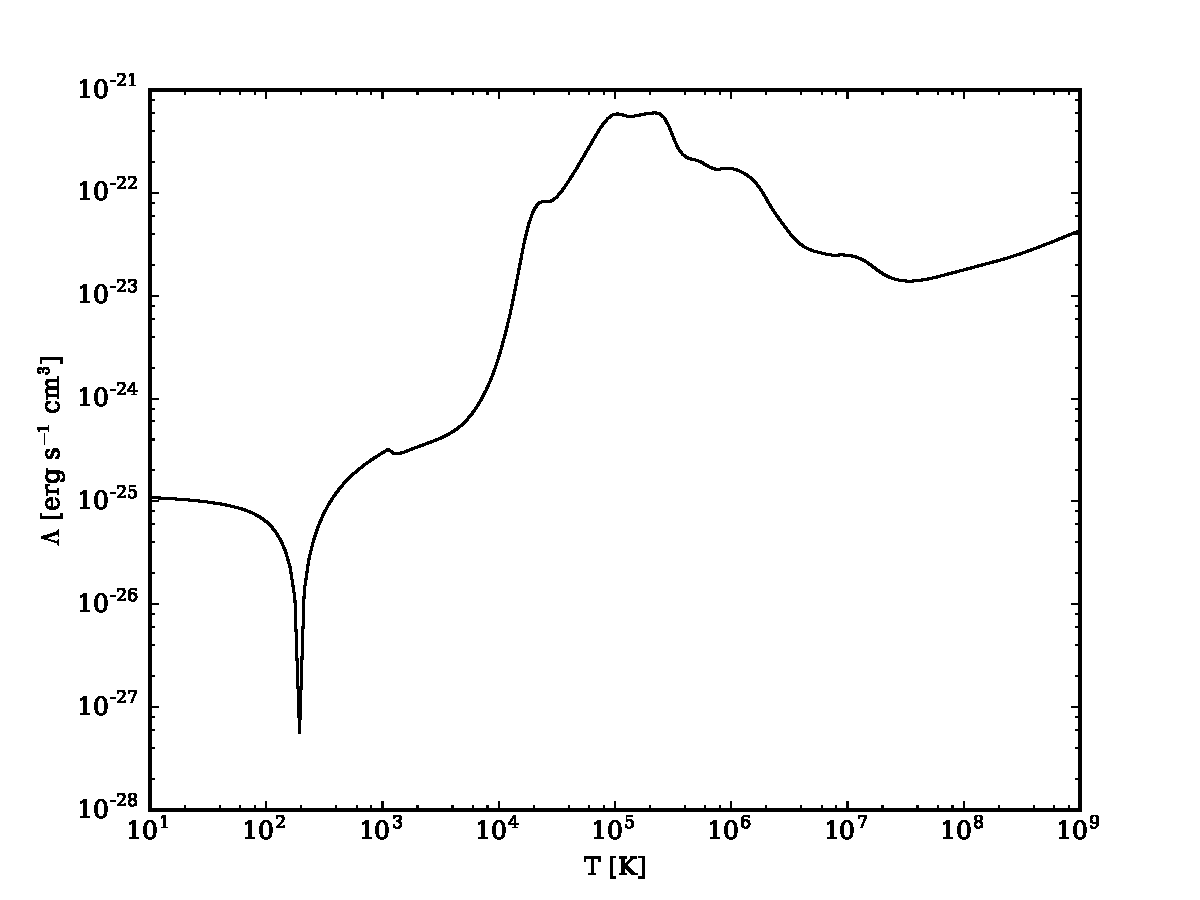
\includegraphics[width=0.45\textwidth]{cooling_rate.pdf}
  \caption{
    Figure output by the default configuration of the cooling rate
    answer test, described in Section \ref{sec:cooling-rate-test},
    showing the equilibrium cooling rate as a function of temperature
    for a solar metallicity gas at a density of 1 amu/cm$^{3}$ with an
    incident radiation field described by the
    \citet{2012ApJ...746..125H} model at z = 0.
  } \label{fig:cooling-rate-test}
\end{figure}

\subsubsection{Answer test: constant density cooling test}
\label{sec:uniform-cooling-test}

The uniform cooling answer test simulates the thermal evolution of a
parcel of gas cooling at constant density.  This test ensures that the
solver properly evolves the internal energy over a period of time.
The test initializes a single-cell fluid container with a density of
0.1 amu/cm$^{3}$ and a temperature of 10$^{6}$ K.  The cell is evolved
for 100 Myr using the \texttt{evolve\_constant\_density} convenience
function with timesteps of 1\% of the cooling time time.  The
resulting evolution is shown in Figure
\ref{fig:uniform-cooling-test}.

\begin{figure}
  \centering
  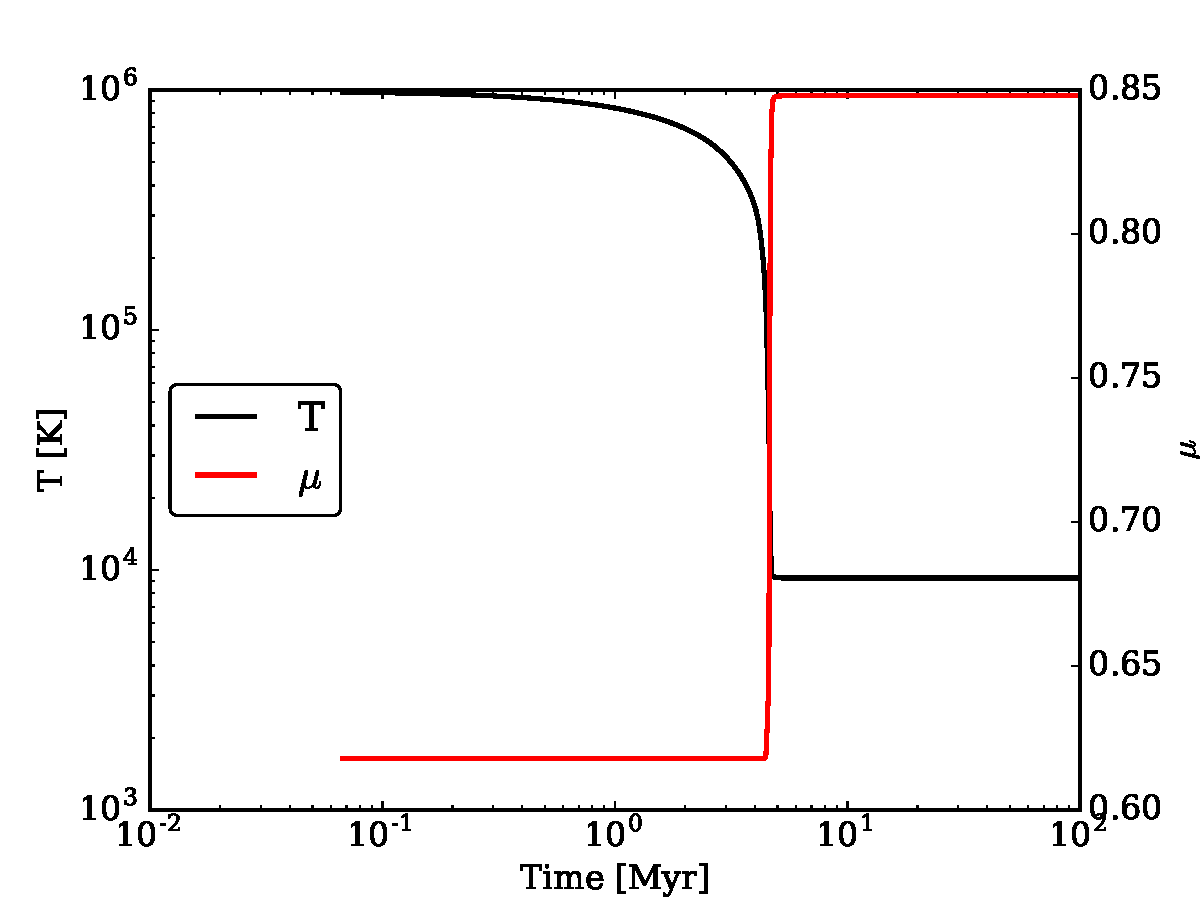
\includegraphics[width=0.45\textwidth]{cooling_cell.pdf}
  \caption{
    Figure output by the uniform cooling answer test, described in
    Section \ref{sec:uniform-cooling-test}, showing the temperature
    (black) and mean molecular weight (red) as a function of time for
    a parcel of gas cooling at constant density.
  } \label{fig:uniform-cooling-test}
\end{figure}

\subsubsection{Answer test: free-fall collapse test}
\label{sec:free-fall-test}

The free-fall collapse answer test simulates the thermal evolution of
a cloud of gas collapsing due to self-gravity.  This test is useful
for ensuring that the non-equilibrium chemistry solver is functioning
properly over a large range in density.  The test creates a
single-cell fluid container with an initial density of 0.1
amu/cm$^{3}$ and an initial temperature of
50,000 K.  Before beginning the free-fall collapse phase, the cloud is
allowed to cool at a constant density to a temperature of 100 K using
the \texttt{evolve\_constant\_density} function described in Section
\ref{sec:pyevolve}.  This allows the gas to settle into an ionization
state that is roughly appropriate for the temperature.  From there, we
evolve the density of the cloud using the \texttt{evolve\_freefall}
function, also discussed in Section \ref{sec:pyevolve}.  This test is
performed using the full non-equilibrium chemistry solver, once at
zero metallicity (Figure \ref{fig:free-fall-test}) and once with a
metallicity of 10$^{-3}$ Z$_{\odot}$.

\begin{figure}
  \centering
  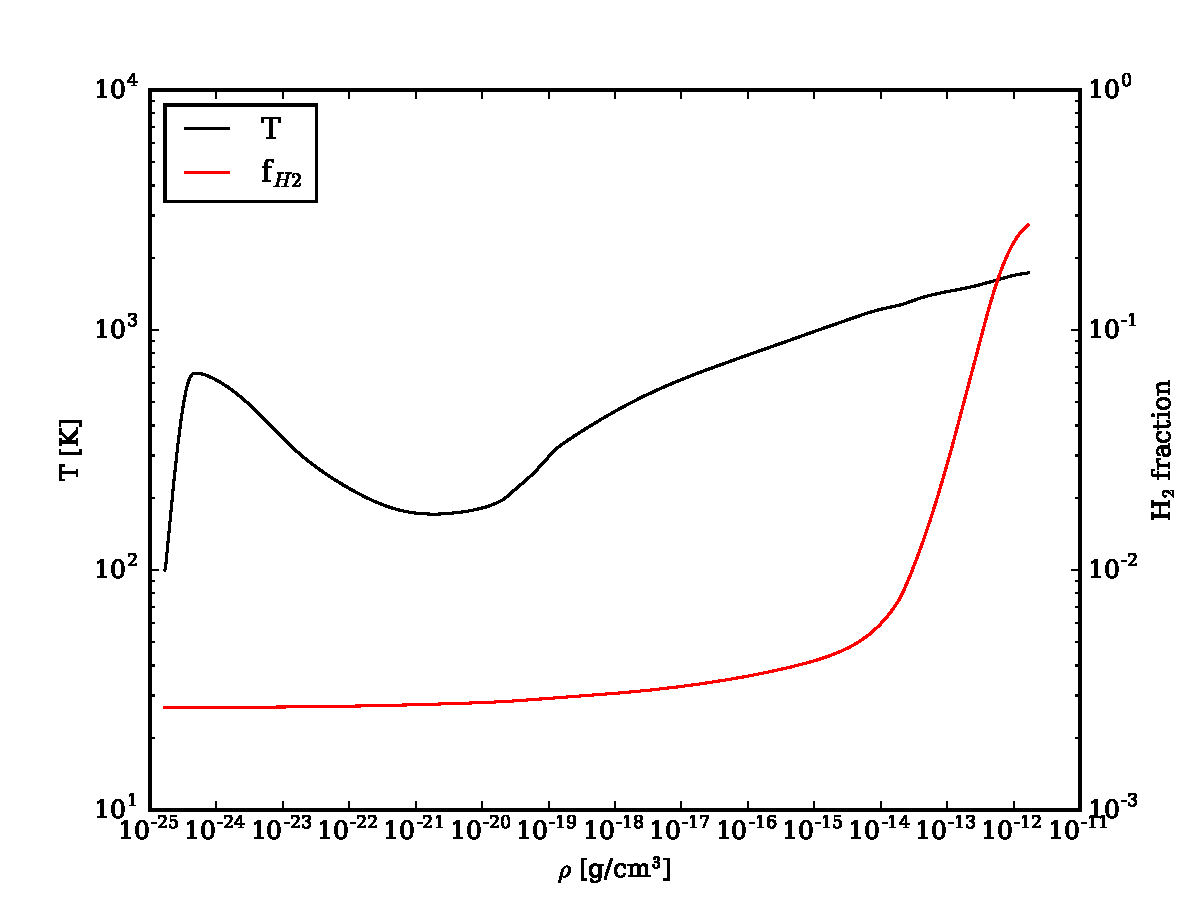
\includegraphics[width=0.45\textwidth]{freefall.pdf}
  \caption{
    Figure output by the default configuration of the free-fall answer
    test, described in Section \ref{sec:free-fall-test}, showing the
    temperature (black) and H$_{2}$ fraction (red) as a function of
    density for a free-fall collapse model of a metal-free gas.
  } \label{fig:free-fall-test}
\end{figure}

\subsection{Performance}


\subsubsection{Optimization Strategy}

Our optimization strategy in the Grackle has two components related to serial and parallel execution.  We begin with single processor optimization.  

The ordinary differential equations that describe chemical and thermal evolution do not use spatial information and so each discretization point (particle or cell) can be evolved independently of the others.  Because of this, the Grackle can be used with a wide variety of codes and applications, and optimization is relatively straightforward.  Our primary technique for single processor optimization is to make good use of cache and (single processor) vectorization.  The API is built around the idea of ``fields" of points (fluid containers) rather than a single point for this reason.  The field can be a single-dimensional contiguous list as might be used for particle-based codes, or a three dimensional grid with inactive ("ghost") points as would be appropriate for grid-based codes.  By taking an entire field, and operating on the field in an order corresponding to the way it is laid out in memory, the code tries to minimize cache misses.  In particular, multi-dimensional arrays are assumed to be fortran-ordered (column-major) and operations are performed in loops over the most rapidly varying index.  Loops are generally also written in a way which facilitates unrolling so that compilers can easily make use of vector operations and prefetching.  Much of the computationally intensive part of the code is written in FORTRAN (in part for historical reasons but in part to take advantage of well-tested FORTRAN compiler loop optimizations).

The second optimization involves taking advantage of parallel computation.  Grackle itself requires no communication and so can easily work as part of a code that uses MPI or some other message passing library to achieve distributed parallelization.  In addition, Grackle supports OpenMP parallelization and thus can easily work with applications adopting a hybrid MPI/OpenMP model.  The OpenMP is implemented by parallelizing over outer j,k loops and giving a thread an i ``slice" to operate on.  This is a natural model for grid-based codes, but some work may be required to get good performance this way with particle based codes (e.g. by artificially splitting a 1D list of particle quantities into a 2D grid).

\subsubsection{Serial Performance}

\begin{figure}
  \centering
  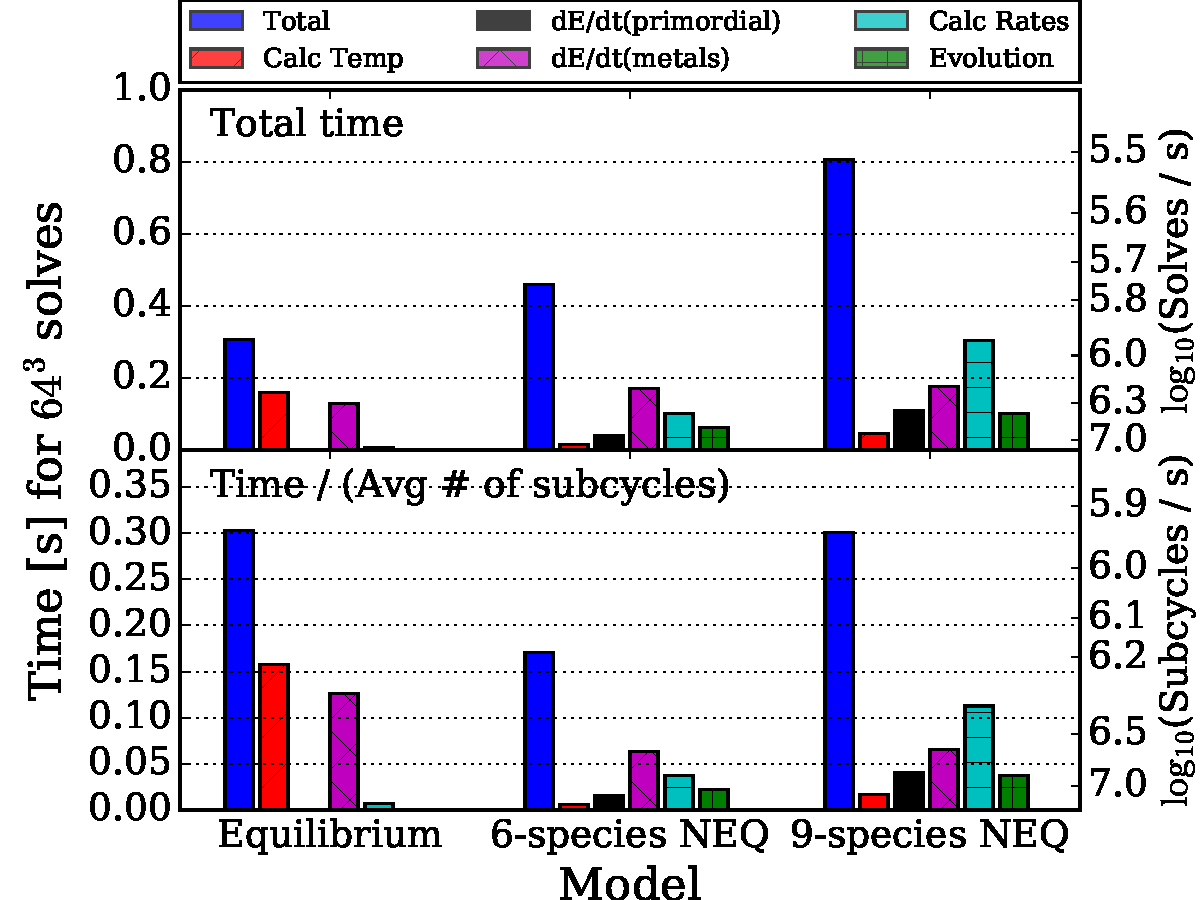
\includegraphics[width=\columnwidth]{performance.pdf}
  \caption{Top panel: Total time to compute the cooling rate test
    (\S\ref{sec:cooling-rate-test}) in $64^3$ fluid containers, using
    the tabulated equilibrium cooling model (left), 6-species
    non-equilibrium model (middle), and 9-species non-equilibrium
    model (right).  The different bars show the time needed for the
    complete solve (blue), the temperature calculation (red), the
    $\dot{e}$ computation due to primordial chemistry (black) and
    metals (magneta), the interpolation of rate coefficients (cyan),
    and the update of the species fractions with backward
    differencing.  Bottom panel: Total time but normalized by the
    average number of subcycles per cell, which demonstrates the
    performance of a single iteration in each solver
    mode.} \label{fig:performance}
\end{figure}

We utilize the cooling rate test (\S\ref{sec:cooling-rate-test}) to
assess the performance of Grackle.  We set up the test with $64^3$
fluid containers with hydrogen number density $n_{\rm H}$, temperature
$T$, and metallicity $Z$ varying in each dimension.  These quantities
are equally log-spaced in the range $\log (n_{\rm H} /
\textrm{cm}^{-3}) = [-1, 3]$, $\log (T/\textrm{K}) = [1, 8]$, and
$\log (Z/Z_\odot) = [-4, 0]$.  All of the fluid containers are
initially neutral.  We run each test with the tabulated solver in
ionization equilibrium and the non-equilibrium solver with the
6-species and 9-species networks on a single core of a desktop
computer with dual Intel Xeon ``Westmere'' E5645 CPUs at 2.4 GHz, each
of which has six cores.  The tests are evolved for 500 yr, which in
most cases is shorter than the cooling time, however, it provides an
ample test for the performance of Grackle.  Because the fluid
containers are not initialized in ionization equilibrium, the first
timestep in the non-equilibrium solvers requires hundreds of subcycles
for the system to converge.  Due to the fact that the non-equilibrium solver
performance is directly tied to the number of subcycles, we do not
include the first three cycles of the tests (which are not representative of
typical use conditions).

% Something about this is an ideal solve, but performance can diminish
% if more difficult (high densities, shocks, or ionization) conditions
% exist.

The top panel of Figure \ref{fig:performance} shows the total time
(blue bars) required for this $64^3$ performance test in each solver
mode.  This is further divided into the time spent in each major
component of Grackle: the calculation of the temperature (red),
$\dot{e}$ from primordial (black) and metal (magenta) species, rate
coefficient interpolation (cyan), and the update of the species
fractions (green).  From a total performance standpoint, the
non-equilibrium solver in the 6-species and 9-species primordial
models require 50\% and 164\% more time than the equilibrium solver,
respectively.  In this test, Grackle can update $8.6 \times 10^5$,
$5.7 \times 10^5$, and $3.2 \times 10^5$ fluid containers per second
for the equilibrium, 6-species and 9-species solvers, respectively.
The computational expense in the equilibrium solver is almost evenly
split between the equilibrium temperature calculation and metal
cooling rates.  The metal cooling rate and rate coefficient
interpolation consume the most compute cycles in the 6-species and
9-species solvers, respectively.  The temperature calculation in the
non-equilibrium solver takes relatively little computation because it
is simply calculated from the pressure and total number density with
no iterative processes.

The cooling rate test represents a fluid in many different
chemo-thermal states, which converge to some equilibrium.  However in
production simulations, there are many ``difficult'' situations, such
as high densities, strong shocks, and strong radiation fields, in
which the equations become stiff and require many subcycles to
complete an entire solve.  Therefore to better gauge the performance
of a single iteration, we show the average time elapsed {\it per
  subcycle} for the same test in the bottom panel of Figure
\ref{fig:performance}.  The equilibrium and non-equilibrium solvers
take an average of 1.01 and 2.67 subcycles per solve, respectively.
Grackle can perform $8.7 \times 10^5$, $1.5 \times 10^6$, and $8.7
\times 10^5$ subcycles per second for the equilibrium, 6-species and
9-species solvers, respectively.  Here we see that the equilibrium
solver actually requires 75\% more time per subcycle as the 6-species
non-equilibrium solver and is equivalent to the performance (per
subcycle) of the 9-species non-equilibrium solver.  In practice, if
any cells require many subcycles to converge to a solution, the call
to Grackle will require additional time per cell than this ideal test,
because the total performance is entirely dependent on the total
number of subcycles performed in one solve, not the number of cells.

\subsubsection{OpenMP Performance}

In addition to the single-processor performance just described, we
characterize the threaded performance of the Grackle.
Figure \ref{fig:omp-perf} shows an OpenMP performance benchmark for both the
non-equilibrium and tabulated functionality, where parallel efficiency is
defined as the ratio of multi-thread to single-thread performance. We
conduct this benchmark on the Campus Cluster of the University of Illinois
at Urbana-Champaign using 20 threads on two Intel Xeon E5-2670 v2 CPUs
at 2.50 GHz, each of which has ten cores. For all time-consuming routines
(i.e., calculating cooling, cooling time, and temperature with the tabulated
solver, and calculating chemistry, cooling, and cooling time with the
non-equilibrium chemistry solver), the parallel efficiency reaches
$\sim 60\%\,\text{--}\,90\%$ for $16^3$ cells and
$\sim 80\%\,\text{--}\,90\%$ for $64^3$ cells. For other computationally cheap
routines, such as calculating pressure, the parallel efficiency is relatively
low. This is not an issue since they take negligible time compared to other
computationally expensive routines.

\begin{figure}
  \centering
  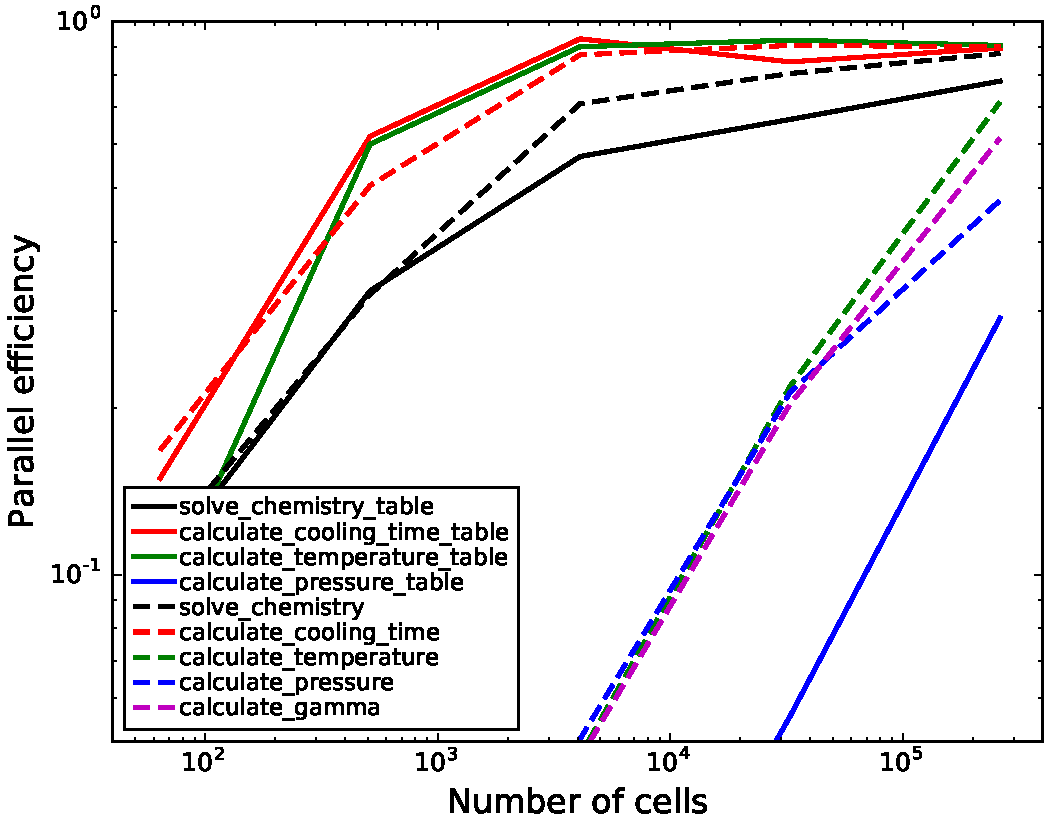
\includegraphics[width=0.45\textwidth]{fig__openmp_performance.pdf}
  \caption{
    OpenMP parallel efficiency using 20 threads as a function of the size of
    the input array. The solid lines show the use of the
    non-equilibrium solver with \texttt{primordial\_chemistry} = 3 and
    the dashed lines show the analogous functions using the tabulated
    solver.  For all time-consuming
    routines, the parallel efficiency reaches $\sim$60\% to 90\% for
    $16^3$ cells and $\sim$80\% to 90\% for $64^3$ cells.
  } \label{fig:omp-perf}
\end{figure}

%%% Local Variables:
%%% mode: latex
%%% TeX-master: "ms"
%%% End:
